% This is "sig-alternate.tex" V1.8 June 2007
% This file should be compiled with V2.3 of "sig-alternate.cls" June 2007
%
% This example file demonstrates the use of the 'sig-alternate.cls'
% V2.3 LaTeX2e document class file. It is for those submitting
% articles to ACM Conference Proceedings WHO DO NOT WISH TO
% STRICTLY ADHERE TO THE SIGS (PUBS-BOARD-ENDORSED) STYLE.
% The 'sig-alternate.cls' file will produce a similar-looking,
% albeit, 'tighter' paper resulting in, invariably, fewer pages.
%
% ----------------------------------------------------------------------------------------------------------------
% This .tex file (and associated .cls V2.3) produces:
%       1) The Permission Statement
%       2) The Conference (location) Info information
%       3) The Copyright Line with ACM data
%       4) NO page numbers
%
% as against the acm_proc_article-sp.cls file which
% DOES NOT produce 1) thru' 3) above.
%
% Using 'sig-alternate.cls' you have control, however, from within
% the source .tex file, over both the CopyrightYear
% (defaulted to 200X) and the ACM Copyright Data
% (defaulted to X-XXXXX-XX-X/XX/XX).
% e.g.
% \CopyrightYear{2007} will cause 2007 to appear in the copyright line.
% \crdata{0-12345-67-8/90/12} will cause 0-12345-67-8/90/12 to appear in the copyright line.
%
% ---------------------------------------------------------------------------------------------------------------
% This .tex source is an example which *does* use
% the .bib file (from which the .bbl file % is produced).
% REMEMBER HOWEVER: After having produced the .bbl file,
% and prior to final submission, you *NEED* to 'insert'
% your .bbl file into your source .tex file so as to provide
% ONE 'self-contained' source file.
%
% ================= IF YOU HAVE QUESTIONS =======================
% Questions regarding the SIGS styles, SIGS policies and
% procedures, Conferences etc. should be sent to
% Adrienne Griscti (griscti@acm.org)
%
% Technical questions _only_ to
% Gerald Murray (murray@acm.org)
% ===============================================================
%
% For tracking purposes - this is V1.8 - June 2007

\documentclass{sig-alternate}
\usepackage{times}
\usepackage{url}
\usepackage{cite}
\usepackage{pstricks}
\usepackage{graphicx} 
\newcommand{\bi}{\begin{itemize}}
\newcommand{\ei}{\end{itemize}}
\newcommand{\be}{\begin{smallenum}}
\newcommand{\ee}{\end{smallenum}}
\newcommand{\tion}[1]{\S\ref{tion:#1}}
\newcommand{\eq}[1]{Equation~\ref{eq:#1}}
\newcommand{\fig}[1]{Figure~\ref{fig:#1}}
\newenvironment{smallitem}
 {\setlength{\topsep}{0pt}
  \setlength{\partopsep}{0pt}
  \setlength{\parskip}{0pt}
  \begin{itemize}
   \setlength{\leftmargin}{.2in}
  \setlength{\parsep}{0pt}
  \setlength{\parskip}{0pt}
  \setlength{\itemsep}{0pt}}
 {\end{itemize}}
\newenvironment{smallenum}
 {\setlength{\topsep}{0pt}
  \setlength{\partopsep}{0pt}
  \setlength{\parskip}{0pt}
  \begin{enumerate}
  \setlength{\leftmargin}{.2in}
  \setlength{\parsep}{0pt}
  \setlength{\parskip}{0pt}
  \setlength{\itemsep}{0pt}}
 {\end{enumerate}}
 
\begin{document}

\conferenceinfo{~}{~}

\title{An Agent Based Wedding Planning Model}


\numberofauthors{1} 
\author{
\alignauthor
Oussama El-Rawas\\
       \affaddr{CPE,  West Virginia University,  USA}\\
       \email{oelrawas@mix.wvu.edu}
}

\maketitle
\begin{abstract}
In this course we have attempted to study agent based development and agent concepts to be applied in software development. In an effort to do just that, we have been presented with an architecture that aims to emulate the concept of agent programming. This Architecture's name is called Actory, and it is implemented in the Smalltalk scripting language. Using Actory, we attempt to model planning a wedding in an agent based manner. Though incomplete, we will present this implementation, along with the projected implementation and learning concepts that were planned, but not implemented. Before that, we will present Actory and how, in this author's opinion, Actory can be improved.
\end{abstract}

\keywords{Agents, BDI, Actory}

\section{Introduction}
Agents in software development have had many different implementations and definitions. These vary from weak agents that have minimal introspective knowledge \cite{woolridge95}, to strong agents \cite{rao95} that have beliefs, intentions and desires umong other possible concepts. The former can be considered a procedure that works with other ``dumb'' procedures for achieving a needed function. The latter is a much more self aware procedure that has:

\be
\item \textbf{Beliefs} concerning its place with respect to the world that it is operating in.
\item \textbf{Desires} that the agent would like to fulfill. These could be thought of as personal goals that aren't necessarily related to the overall goal.
\item \textbf{Intentions} that is the driving force behind most of the agent's actions, and which is the final intended goal of the agent, possibly shared by peer agents.
\ee

These agent concepts are briefly explained in \cite{me02m} along with other agent concepts. Going into this course, one of our objectives was to learn and critique these Agent-based programming methods in an attempt to understand further what agents are, or even what they ought to be. For this the above and other references were used. We also aimed to demostrate Agent oriented programming methods, using an architecture called Actory as the basis of our Agent oriented programs. Using that basis, we moved on to making an Agent based system for wedding planning loosely derived from personal experience planning a wedding. 

In what follows, we will briefly explain Actory, followed by an explanation of our wedding planning model and how that fits into Actory and Agent oriented programming.

\section{The Actory Model}
In this section we will briefly present the architecture of the Actory model. We will also present how, in our opinion, Actory interprets the concept of strong agency.

\begin{figure}
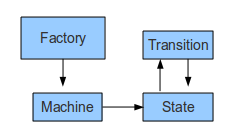
\includegraphics{Actory.png}
\caption{A simple depiction of the Actory architecture}
\end{figure}\label{fig:actory}

The general hierarchy in Actory, depicted in \fig{actory}, can be described as follows starting with the lowest in that heirarchy:

\bi
\item \textbf{Transitions} are the very basic structure of Actory that include the core of the logic and actions. Transitions are defined by their starting and ending states, the condition under which they fire (the guard), and the side effects or actions the will be executed. Transitions are specific to a Machine in the current state of Actory.
\item \textbf{States} are the condition of the Machine, and can be defined to affect a Machine in different ways, whether or not that includes executing actions. Defined States can be used by any Machine, but can only be used by a Machine if it is included in that Machine's Transitions.
\item \textbf{Machine} is the main actor in Actory (pun not intended), and seeks to achieve a goal or at least try to. This is done by going through Transitions until it reaches and end state.
\item \textbf{Factory} Factory is the playground where the Machines operate, and is able to store data to be used by all the Machines. A Factory can be used as a world model, or to represent a particular function that is separate from the main goal function, i.e. Transitions can start new Factories which Machines to achieve some side goal.
\ei

For our purposes, we consider Machines to be the cooperative agents working in a world model defined in Actory. States are considered to the Machines' belief, or internal state, where being in a state allows a Machine to use certain Transitions. As such, Transitions as a whole are considered to be the expression of a Machine's desires. These Transitions also work towards a common goal in the Machines, this goal being the collective Intention within the factory. By assuming the following representation of BDI concepts in Actory, we moved on to design and implement the wedding planning model.

\section{The Wedding Planning Model}
Based on Actory, we implemented an agent based wedding planning model. This model includes definitions of people, who are the individual social agents implemented as machines within Actory, as well as custom states they can be in. There's also a customized wedding factory, and some task classes. We will present this briefly in what follows. Note that the fitness function for this model is simply the sum of all the happiness of all the Machines (which represent people). Further tweaking and weighting
fo the fitness function has not been explored.

\subsection{People}
There are several types of people defined as machine types with designated states and transitions. Note that here people are defined using inheritance, where a more complex person takes on properties of the previous person type in addition to other properties specific to that person type. These properties are expressed in terms of specific methods and transitions.

\bi
\item \textbf{Guest} is a person that has happiness. The only role of this machine is to wait for the wedding and to attend and hopefully be happy.
\item \textbf{Close Friend or Family (CFF)} is a Guest that is also able to be busy or idle. If the latter is true, they could offer to help with a task that is running behind schedule.
\item \textbf{Bridal Party (BP)} is a Close Friend or Family that is also capable of taking charge of a task. They are also able to ask for help should they realize that the task they are in charge of is behind schedule.
\item \textbf{Parents OF Bride/Groom (POB/POG)} are a Bridal Party who are also responsible for distributing funds necessary for implementing the different tasks.
\item \textbf{BrideGroom} are a Bridal Party, except they are also able to choose the variety of tasks to be implemented from the list available (for example picking which reception alternative to be implemented.
\ei

Here one weakness of Actory is revealed, where machines are unable to share common transitions. As such, many transitions had to be repeated in multiple machines.

\subsection{States}
There are four main states that are used in this model for the machines:

\bi
\item \textbf{Happy} achieved when people are enjoying themselves, i.e. eating, seeing the nice decoration.
\item \textbf{Idle} Just waiting around doing nothing, possibly willing to offer assistance.
\item \textbf{Busy} Unable to offer assistance or already working on or helping with a task.
\item \textbf{BusyNeedHelp} Unable to offer assistance, but also in need of assistance.
\ei

These states determine which subset of available transitions are available.

\subsection{Wedding Factory}
Wedding is a customized Factory that also saves the available alternatives to tasks. These are used by the bride and groom to pick from. Wedding also has the queue of tasks that need help for those persons that can help to choose from. Generally, the Wedding Factory has everything that needs to be shared globally to all Machines, and therefore through which they communication. This reveals another weakness Actory where machines can't communicate directly.

\subsection{Tasks}
This class simply defines Tasks, with properties such as time needed, time to completion and cost, in addition to the amount of people working on the Task. There are two subtypes: food which adds number of options and portions, and ceremony which adds the ceremony length.

\section{Conclusions}
In this project, we attempted to implement strong agency into a wedding planning model based on an architecture called Actory. Unfortunately this implementation was not completed, preventing us from having complete baseline results.

\bibliographystyle{abbrv}
\bibliography{refs} 

%\appendix

\end{document}
